\newgeometry{left=0.5cm,right=0.5cm,top=1cm,bottom=1cm}
\begin{multicols}{2}
\setstretch{0.9}
\begin{enumerate}[label=\textbf{\arabic*.},start=4]
\addtolength{\itemindent}{1.5cm}
\setlength\itemsep{1pt}
\item  Использовать условия, при которых оба корня трехчлена.
$$  f(x)=x^2+x+a $$
больше числа $a$  , а именно,
$$1-4a\geq 0, a^2+2a \geq -\dfrac{1}{2}>a.$$
Ответ $ a<-2.$
\item $a=0$ и $a=2$.
\item $\dfrac{H}{2}.$
\item Наименьшее значение функции $x^2+1$ равно 1 и достигается при $x=0$. Поэтому
$$x^2+1>\cos{x}$$
при всех $x\neq 0$. Значение $x=0$ - корень уравнения
\item Использовать условия, при которых оба корня квадратного трехчлена
\begin{center}
$f(x)=x^2+mx+m^2+6m$
\end{center}
лежат вне промежутка $1<x<2$, а именно, $f(1)<0, f(2)<0$.\\
Следовательно, нужно найти значение $m$, удовлятворяющее одновременно двум неравенствам
\begin{equation}
	m^2+7m+1<0,
	m^2+8m+4>0.
\end{equation}
Решая эти неравенства и отбирая их общие решения, находим ответ:
$$\dfrac{-7-3\sqrt{5}}{2}<m<-4+2\sqrt{3}$$.
\item $\dfrac{2v_0^2\sin{2\alpha}}{g}-S $.
\end{enumerate}
\begin{center}
\addtolength{\parindent}{1.5cm}
\color{red}
\textbf{
К статье \\*
\flqq Шахматно-математические заметки\frqq } \\*
(см. Квант № 8)
\end{center}
\begin{enumerate}[label=\textbf{\arabic*.},start=1]
\setlength\itemsep{1pt}
\addtolength{\itemindent}{1.5cm}
\item Достаточно заметить, что каждая фигура содержит либо 3 белых поля, либо 3 черных, а всего таких фигур должно быт 25.
\item Легко убедиться, что при любом покрытии каждое тримино содержит ровно одно поле, через которое проходит красная линия и ровно одно, черек которое проходит черная линия. Поскольку \flqq красных\frqq  и \flqq черных\frqq  полей по 22, а тримино - 21, то не покрыто одно \flqq красно-черное\frqq  поле из 
\begin{center}
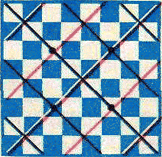
\includegraphics{pic}
\end{center}
четырех, отмеченных на рисунке. Проверьте, что соответствующие покрытия существуют.
\item Напишем на каждом поле доски номер горизонтали, в которой это поле стоит. Проверьте, что каждое тримино покрывает поля с суммой чисел, делящейся на 3, а нам надо покрыть поля с суммой чисел 296, дающей при делении на 3 остаток 2.
\item а) Нет. \flqq Белая\frqq  пешка (пешка, стоящая на белом поле) при вторичной расстановке должна стать \flqq черной\frqq , а \flqq черная\frqq  - \flqq белой\frqq . Значит, число \flqq белых\frqq  пешек равно числу \flqq черных\frqq , что противоречит нечетности доски.\\
\addtolength{\parindent}{1.5cm}
б) Нет. Докажите, что пешки, стоящие на крайней левой вертикали, остались на месте (из a1 в a8 можно пройти по 6 смежным полям). Дальше рассмотрите поля b1 и b8.
\end{enumerate}
\end{multicols}
\begin{center}
\addtolength{\parindent}{1.5cm}
\color{red}
\textbf{
К заметке\\*
\flqq Еще несколько задач Васи Смекалкина\frqq }\\*
(см. "Квант" № 8, 3-я страница обложки)
\end{center}
\begin{enumerate}[label=\textbf{\arabic*.},start=1]
\addtolength{\itemindent}{1.5cm}
\item Составим таблицу разностей чисел данной последовательности (между соседними числами запишем их разность).В третьей строчке получится последовательность степеной двойчки. После этого ясно, как продолжить таблицу.\\
\begin{tabular}{ |p{0.75cm}|p{0.75cm}|p{0.75cm}|p{0.75cm}|p{0.75cm}|p{0.75cm}|p{0.75cm}|p{0.75cm}|p{0.75cm}|p{0.75cm}|p{0.75cm}|p{0.75cm}|p{0.75cm}|p{0.75cm}|p{0.75cm}|p{0.75cm}| }
\hline 
 4&  & 7 &  & 12 & & 21 & & 38 & & \color{blue}71 & & \color{blue}126& &\color{blue}245 &\color{blue}...\\
\hline
  & \multicolumn{3}{c|}{35}&  &9 & & 17 & & \color{blue}33 & &\color{blue} 55 & &\color{blue}119 &\color{blue} ...&\\
\hline
  &  &  2 & &4 & &8 & & \color{blue}16 & &\color{blue}32 & & \color{blue}64  &\color{blue}...& &\\
\hline
\end{tabular}
\end{enumerate}